\documentclass{article}
\usepackage{amsmath,amssymb,braket,bbm,graphicx}
\usepackage[margin=2.5cm]{geometry}

\begin{document}
	
\noindent
Consider the LSWT Hamiltonian $\mathcal H_2 = \sum_{kn} \epsilon_{kn} \alpha_{kn}^\dagger \alpha_{kn}$.
Suppose we have computed the following vertex factors (quantum matrix elements) for fixed momentum $\vec k$ and arbitrary momentum $\vec q \in \mathrm{BZ}$:
\begin{gather}
	g^{---}_{kq,nml} \alpha_{-k-q,n} \alpha_{qm} \alpha_{kl} \hspace{1.5cm}
	g^{+--}_{kq,nml} \alpha_{k+q,n}^\dagger \alpha_{q,m} \alpha_{kl} \hspace{1.5cm}
	g^{++-}_{kq,nml} \alpha_{k+q,n}^\dagger \alpha_{-q,m}^\dagger \alpha_{kl} \hspace{1.5cm}
	\\
	\tilde g^{-}_{n} \alpha_{0n} \hspace{1.5cm}
	\tilde h^{+-}_{k,nm} \alpha_{kn}^\dagger \alpha_{km}
\end{gather}
The first three vertex factors are due to the cubic vertex and are of order $\mathcal O(\sqrt S)$.
The fourth vertex is a commutator term coming from normal-ordering the cubic vertex and is of order $\mathcal O(\sqrt S)$.
The fifth vertex is a commutator term coming from normal-ordering the quartic vertex and is of order $\mathcal O(S^0)$. \\
All vertices are normal-ordered and symmetrized in their particle/hole degrees of freedom.
%Consider the following magnon Hamiltonian:
%\begin{align}
%	\mathcal H &= E_\mathrm{gs} + \mathcal H^{comm}_1 + \mathcal H_2 + \mathcal H^{comm}_2 + \mathcal H_3 + \mathcal H_4
%\end{align}
%where
%\begin{align}
%	\mathcal H_2 &= \sum_{k,n} \epsilon_{k;n} \alpha_{k;n}^\dagger \alpha_{k;n} \\
%%
%	\mathcal H_3 &= \frac{\sqrt S}{\sqrt N} \sum_{kq,nml} \left( g^{---}_{kq;nml} \alpha_{-k-q;n} \alpha_{q;m} \alpha_{k;l} + g^{++-}_{kq;nml} \alpha_{k+q;n}^\dagger \alpha_{-q,m}^\dagger \alpha_{k,l} + \dots \right)
%\end{align}
\\
\\
The Dyson equation reads
\begin{align}
	G = G^0 + G^0 \Sigma G
\end{align}
with the non-interacting propagator $G^0$, the interacting propagator $G$ and the self-energy $\Sigma$.
Diagramatically, we assign a negative propagator to every line due to the sign the propagator $G(\tau) \sim -\braket{T_\tau a(\tau) a^\dagger(0)}$ is defined with. We obtain: \\
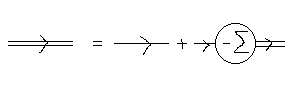
\includegraphics{Dyson_equation.png} \\
So the one-particle irreducible diagrams we draw acually give us the \emph{negative} of the self-energy.
	
\section{One-Loop}
	
\noindent
Compute exact expressions for all one-loop Feynman diagrams.
We will need the bosonic Matsubara sum
\begin{align}
	\frac{1}{\beta} \sum_{i\omega} \frac{1}{(i\omega - \xi_1) (i\omega - \xi_2)} = -\frac{n_B(\xi_1) - n_B(\xi_2)}{\xi_1 - \xi_2} \qquad (*)
\end{align}
We will also use that $n_B(i\omega + z) = n_B(z)$ for bosonic Matsubara frequencies $i\omega$, and that $n_B(-z) = -1 - n_B(z)$.

\subsection{Particle-Particle Bubble}
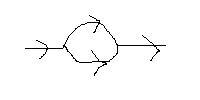
\includegraphics{Feynman_pp_bubble.png} \\
By the Feynman rules, we find the following expression:
\begin{align}
	\Sigma_{nm}^\mathrm{pp-bubble}(i\Omega, \vec k) &= -\frac{2}{\beta N} \sum_{\vec q,ll'} g^{++-}_{kq,ll'n} (g^{++-}_{kq,ll'm})^* \sum_{i\omega} \frac{1}{(i\omega - \epsilon_{-q,l}) (i\Omega - i\omega - \epsilon_{k+q,l'})} \\
%
	&\overset{(*)}{=} -\frac{2}{N} \sum_{\vec q,ll'} g^{++-}_{kq,ll'n} (g^{++-}_{kq,ll'm})^* \, \frac{n_B(\epsilon_{-q,l}) - n_B(i\Omega - \epsilon_{k+q,l'})}{\epsilon_{-q,l} - (i\Omega - \epsilon_{k+q,l'})} \\
%
	&= \frac{2}{N} \sum_{\vec q,ll'} g^{++-}_{kq,ll'n} (g^{++-}_{kq,ll'm})^* \, \frac{1 + n_B(\epsilon_{-q,l}) + n_B(\epsilon_{k+q,l'})}{i\Omega - \epsilon_{-q,l} - \epsilon_{k+q,l'}} \\
%
	&\overset{T\to 0}{\longrightarrow} \frac{2}{N} \sum_{\vec q,ll'} \frac{g^{++-}_{kq,ll'n} (g^{++-}_{kq,ll'm})^*}{i\Omega - \epsilon_{-q,l} - \epsilon_{k+q,l'}}
\end{align}
The symmetry factor $2$ comes about because there are two possible ways to wire the loop.

\subsection{Particle-Hole Bubble}
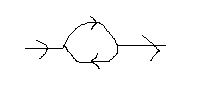
\includegraphics{Feynman_ph_bubble.png} \\
By the Feynman rules, we find the following expression:
\begin{align}
	\Sigma_{nm}^\mathrm{ph-bubble}(i\Omega, \vec k) &= -\frac{1}{\beta N} \sum_{\vec q,ll'} g^{+--}_{kq,ll'n} (g^{+--}_{kq,ll'm})^* \sum_{i\omega} \frac{1}{(i\omega - \epsilon_{q,l}) (i\Omega + i\omega - \epsilon_{k+q,l'})} \\
	%
	&\overset{(*)}{=} \frac{1}{N} \sum_{\vec q,ll'} g^{+--}_{kq,ll'n} (g^{+--}_{kq,ll'm})^* \, \frac{n_B(\epsilon_{q,l}) - n_B(-i\Omega + \epsilon_{k+q,l'})}{\epsilon_{q,l} - (-i\Omega + \epsilon_{k+q,l'})} \\
	%
	&= \frac{1}{N} \sum_{\vec q,ll'} g^{+--}_{kq,ll'n} (g^{+--}_{kq,ll'm})^* \, \frac{n_B(\epsilon_{q,l}) - n_B(\epsilon_{k+q,l'})}{i\Omega + \epsilon_{q,l} - \epsilon_{k+q,l'}} \\
	%
	&\overset{T\to 0}{\longrightarrow} 0
\end{align}
The symmetry factor is $1$ (TODO) because there is exactly one possible way to wire the loop.

\subsection{Hole-Hole Bubble}
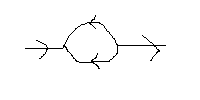
\includegraphics{Feynman_hh_bubble.png} \\
By the Feynman rules, we find the following expression:
\begin{align}
	\Sigma_{nm}^\mathrm{hh-bubble}(i\Omega, \vec k) &= -\frac{2}{\beta N} \sum_{\vec q,ll'} g^{---}_{kq,ll'n} (g^{---}_{kq,ll'm})^* \sum_{i\omega} \frac{1}{(i\omega - \epsilon_{q,l}) (-i\Omega - i\omega - \epsilon_{-k-q,l'})} \\
	%
	&\overset{(*)}{=} -\frac{2}{N} \sum_{\vec q,ll'} g^{---}_{kq,ll'n} (g^{---}_{kq,ll'm})^* \, \frac{n_B(\epsilon_{q,l}) - n_B(-i\Omega - \epsilon_{-k-q,l'})}{\epsilon_{q,l} - (-i\Omega - \epsilon_{-k-q,l'})} \\
	%
	&= -\frac{2}{N} \sum_{\vec q,ll'} g^{---}_{kq,ll'n} (g^{---}_{kq,ll'm})^* \, \frac{1 + n_B(\epsilon_{q,l}) + n_B(\epsilon_{-k-q,l'})}{i\Omega + \epsilon_{q,l} + \epsilon_{-k-q,l'}} \\
	%
	&\overset{T\to 0}{\longrightarrow} -\frac{2}{N} \sum_{\vec q,ll'} \frac{g^{---}_{kq,ll'n} (g^{---}_{kq,ll'm})^*}{i\Omega + \epsilon_{q,l} + \epsilon_{-k-q,l'}}
\end{align}
The symmetry factor $2$ (TODO!) comes about because there are two possible ways to wire the loop.

\subsection{Particle Stub}
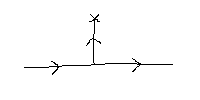
\includegraphics{Feynman_p_stub.png} \\
By the Feynman rules, we find the following expression:
\begin{align}
	\Sigma_{nm}^\mathrm{p-stub}(\vec k) &= -\frac{1}{N} \sum_{l} \frac{g^{++-}_{k0,mln} \tilde g^{-}_{l}}{-\epsilon_{0l}}
%
	= \frac{1}{N} \sum_{l} \frac{g^{++-}_{k0,mln} \tilde g^{-}_{l}}{\epsilon_{0l}}
\end{align}
The symmetry factor is $1$ (TODO) because there is exactly one possible way to wire the vertices together. \\
Note that the diagram is frequency-independent.

\subsection{Hole Stub}
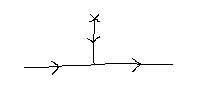
\includegraphics{Feynman_h_stub.png} \\
By the Feynman rules, we find the following expression:
\begin{align}
	\Sigma_{nm}^\mathrm{h-stub}(\vec k) &= -\frac{1}{N} \sum_{l} \frac{g^{+--}_{k0,mln} \tilde g^{+}_{l}}{-\epsilon_{0l}}
	%
	= \frac{1}{N} \sum_{l} \frac{g^{+--}_{k0,mln} \tilde g^{+}_{l}}{\epsilon_{0l}}
\end{align}
The symmetry factor is $1$ (TODO) because there is exactly one possible way to wire the vertices together. \\
Note that the diagram is frequency-independent.

\subsection{Quadratic Insertion}
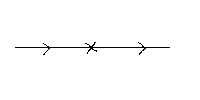
\includegraphics{Feynman_quadratic_insertion.png} \\
By the Feynman rules, we find the following expression:
\begin{align}
	\Sigma_{nm}^\mathrm{quadratic-insertion}(\vec k) &= -\frac{1}{N} \tilde h^{+-}_{k,nm}
\end{align}
The symmetry factor is $1$ because there is exactly one possible way to wire the external legs to the vertex. \\
Note that the diagram is frequency-independent.


\end{document}